\documentclass{article}
\usepackage[T1]{fontenc}
\usepackage{lmodern}
\usepackage{graphicx}
\usepackage{amsmath,amssymb}
\usepackage[a4paper,margin=2cm]{geometry}
\usepackage[absolute,overlay]{textpos}
\setlength{\TPHorizModule}{1mm}
\setlength{\TPVertModule}{1mm}
\usepackage[indonesian]{babel}
\usepackage{hyperref}
\setlength{\emergencystretch}{2em}
% unit: Halaman 71

\begin{document}

% === Halaman 71 (llm) ===

\section*{Beberapa kesalahan umum karena tidak paham kriptografi}

\vspace{187.11mm}

\begin{itemize}
    \item Menganggap enkripsi = encoding, hashing, tokenisasi.
    \item Tidak paham perbedaan \textit{symmetric encryption} dan \textit{asymmetric encryption}, kapan menggunakan \textit{symmetric} dan kapan menggunakan \textit{asymmetric encryption}
\end{itemize}

\vspace{10mm}

Sumber gambar: Slide kuliah tamu dari Burman Noviansyah

% deskripsi: Meme yang menunjukkan kebingungan antara enkripsi, hashing, dan Base64 menggunakan potongan gambar karakter film.
% bbox normalisasi: [0.6210, 0.2780, 0.9760, 0.9080]
\begin{textblock*}{74.55mm}(130.41mm,82.57mm)
\noindent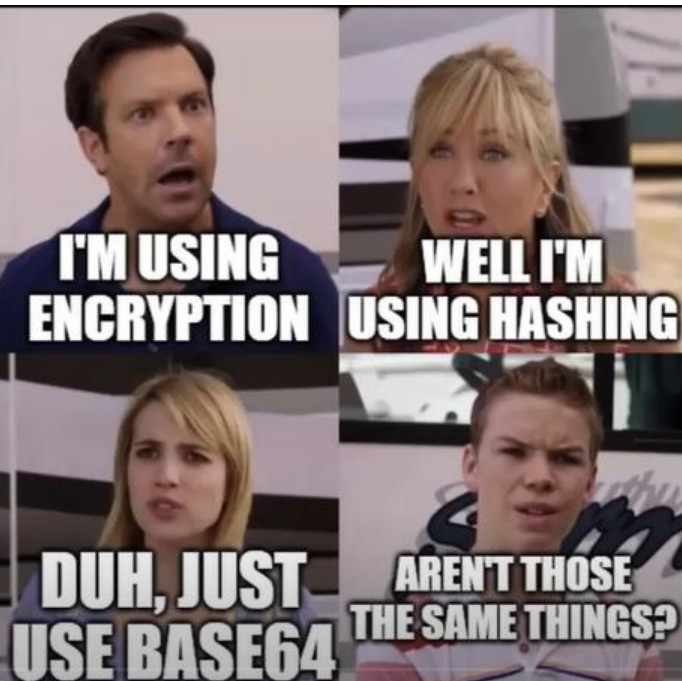
\includegraphics[width=74.55mm,height=187.11mm]{../../images/llm/page_071_img_01.png}%
\end{textblock*}

\end{document}
